\begin{frame}{}
    \LARGE NLP: \textbf{Attention Mechanism}
\end{frame}

\begin{frame}{Sequence to Sequence Learning}
    \begin{figure}
        \centering
        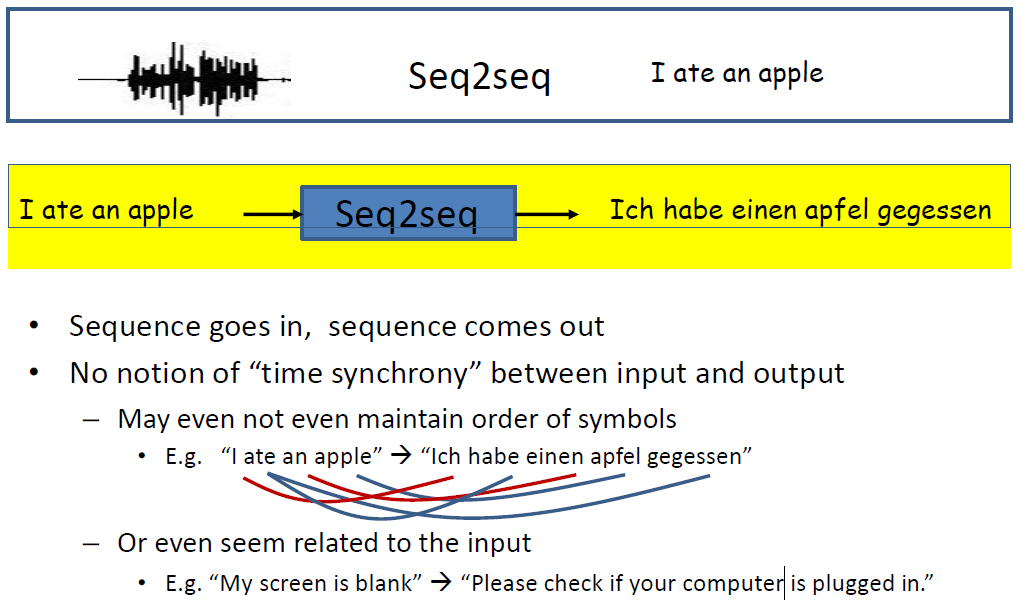
\includegraphics[width=\linewidth, height=0.9\textheight,keepaspectratio]{images/nlp/seq2seq.png}
    \end{figure}
\end{frame}

\begin{frame}[allowframebreaks]{Modelling the Problem}
    \begin{figure}
        \centering
        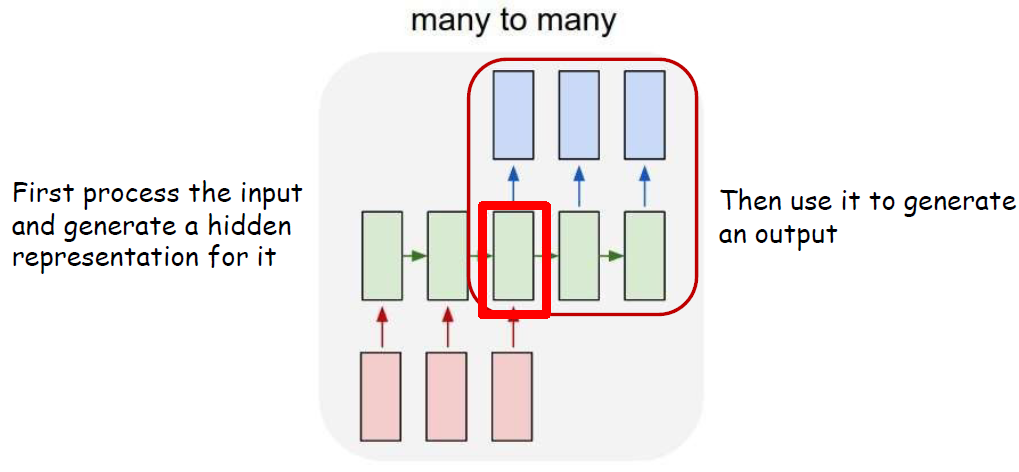
\includegraphics[width=\linewidth, height=0.7\textheight,keepaspectratio]{images/nlp/problem-modelling.png}
    \end{figure}

    \textbf{Delayed Sequence to Sequence Problem:}

    \textbf{Problem}: Each word that is output depends only on the current hidden state, and not on previous outputs.

    \framebreak

    \begin{figure}
        \centering
        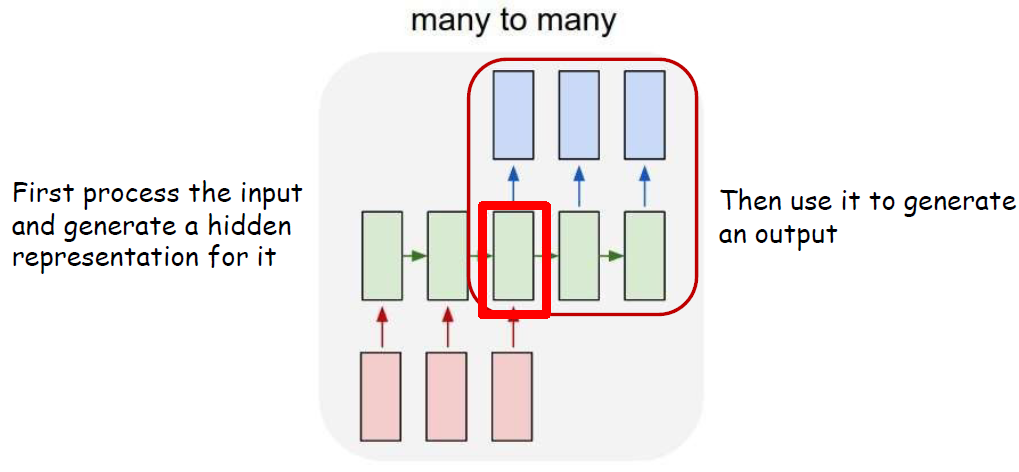
\includegraphics[width=\linewidth, height=0.7\textheight,keepaspectratio]{images/nlp/problem-modelling.png}
    \end{figure}

    \textbf{Delayed Sequence to Sequence Problem:}

    Delayed \textit{self-referencing} sequence-to-sequence: Each word that is output depends on the current hidden state, and also on previous outputs.

\end{frame}

\begin{frame}{The “simple” translation model}
    \begin{figure}
        \centering
        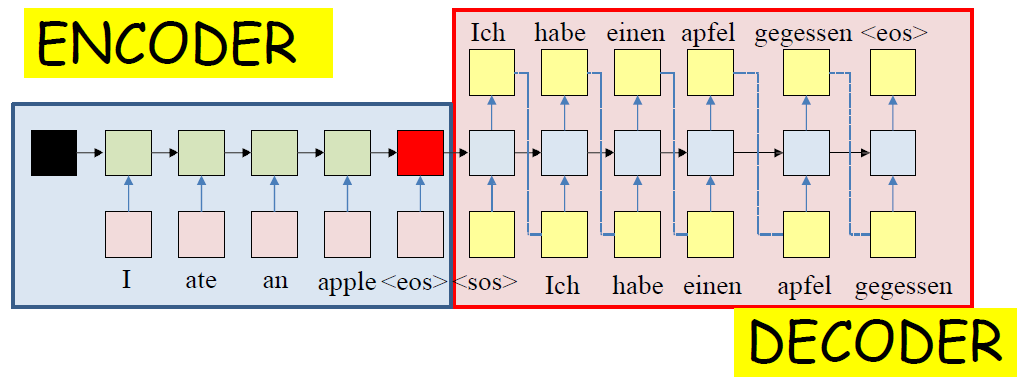
\includegraphics[width=\linewidth, height=0.7\textheight,keepaspectratio]{images/nlp/simple-transition-model.png}
    \end{figure}

    The recurrent structure that:
    \begin{itemize}
        \item extracts the hidden representation from the input sequence is the \textbf{encoder}.
        \item utilizes this representation to produce the output sequence is the \textbf{decoder}.
    \end{itemize}
\end{frame}

\begin{frame}{Problems with the “simple” translation model}
    \begin{figure}
        \centering
        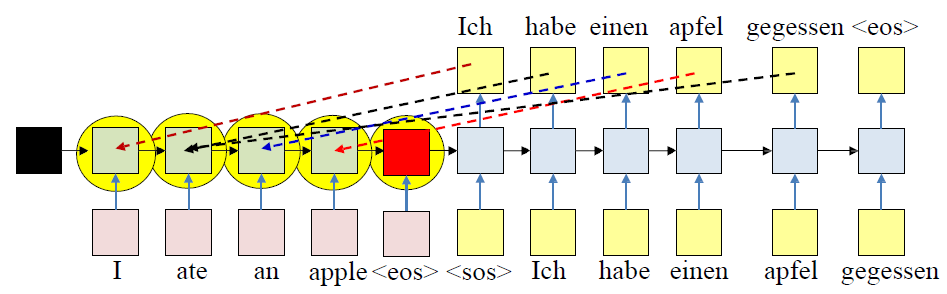
\includegraphics[width=\linewidth, height=0.7\textheight,keepaspectratio]{images/nlp/problem-simple-transition.png}
    \end{figure}
    \begin{itemize}
        \item The model has to compress all the information from the input sequence into a single fixed-size vector.
        \item This can lead to loss of important information, especially for long sequences.
        \item The model struggles with long-range dependencies and context retention.
    \end{itemize}
\end{frame}

\begin{frame}{Attention Models}
    \begin{figure}
        \centering
        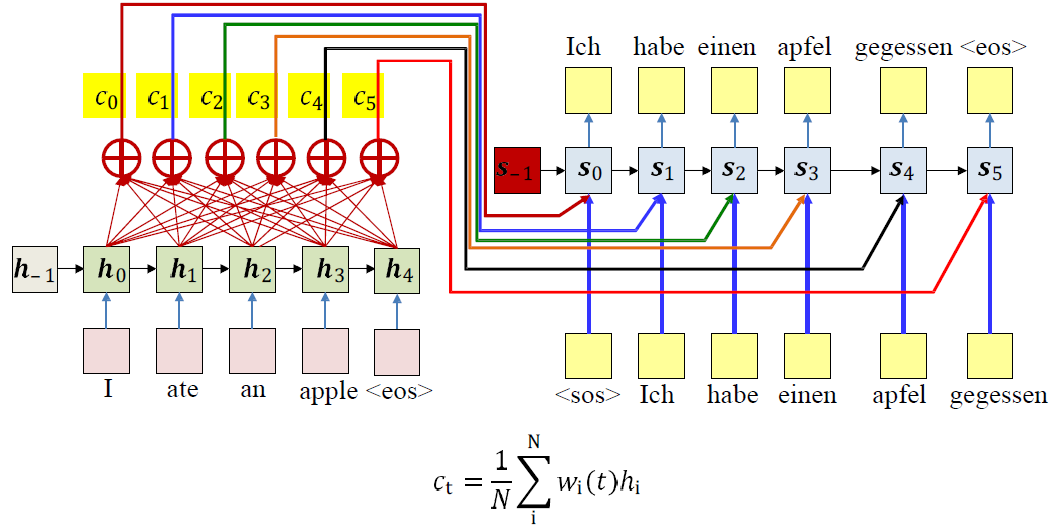
\includegraphics[width=\linewidth, height=0.6\textheight,keepaspectratio]{images/nlp/attention-models.png}
    \end{figure}
    \begin{itemize}
        \setlength{\itemsep}{-0.5em}
        \item \textbf{Attention weights:} The weights $w_i(t)$ are dynamically computed as functions of the decoder state and the encoder outputs.
        \item<2-> \textbf{Intuition:} If the model is well-trained, these weights will automatically “highlight” the most relevant parts of the input sequence for each output step.
        \item<3-> \textbf{\large How are they computed?}
    \end{itemize}
\end{frame}

\begin{frame}{Attention Weights at time $t$}
    \begin{figure}
        \centering
        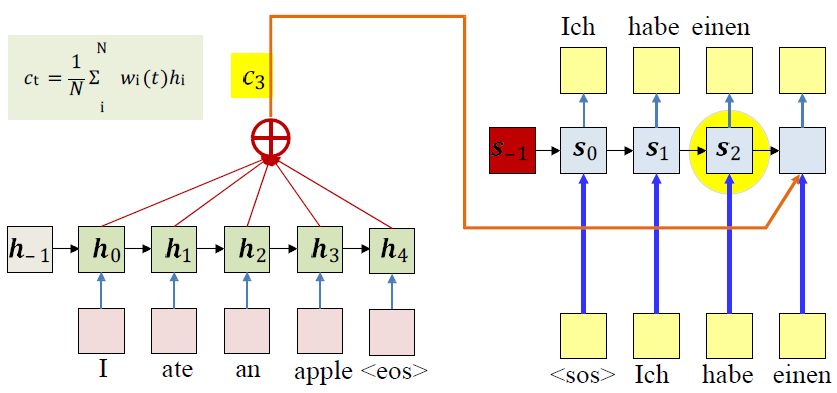
\includegraphics[width=\linewidth, height=0.9\textheight,keepaspectratio]{images/nlp/attention-weights.png}
    \end{figure}
\end{frame}
\begin{frame}{Attention Weights at time $t$}
    \begin{itemize}
        \setlength{\itemsep}{-0.5em}
        \item \textbf{What do attention weights do?} They tell the model which input words to pay more attention to when making each output word.
        \item<2-> The \textbf{attention} weight $w_i(t)$ determines how much focus the model places on the $i$-th input position when producing the output at time $t$.
        \item<3-> The primary information used to compute $w_i(t)$ is the encoder hidden state $h_i$ (at input position $i$) and the decoder state $s_{t-1}$ (at the previous output time step).
        \item<4-> The attention score is typically computed as:
            \[
            w_i(t) = a(h_i, s_{t-1})
            \]
            where $a(\cdot)$ is a function (such as a dot product, additive, or other scoring function).
        \item<5-> Sometimes, the input word at time $t$ is also used, but often omitted for simplicity.
    \end{itemize}
\end{frame}

\begin{frame}[allowframebreaks]{Requirement on attention weights}
    \begin{figure}
        \centering
        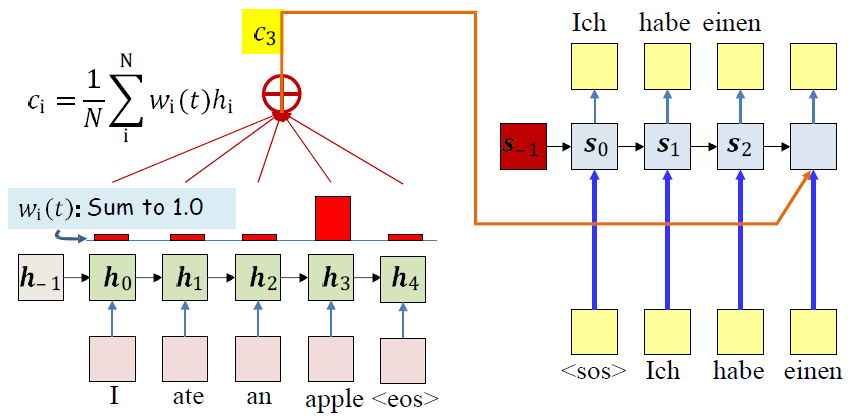
\includegraphics[width=\linewidth, height=0.6\textheight,keepaspectratio]{images/nlp/attention-weights-requirement.png}
    \end{figure}
    \begin{itemize}
        \setlength{\itemsep}{-0.5em}
        \item The attention weights $w_i(t)$ must satisfy the following properties:
        \begin{itemize}
            \item They are non-negative: $w_i(t) \geq 0$ for all $i$.
            \item They sum to 1: $\sum_{i=1}^{n} w_i(t) = 1$, where $n$ is the length of the input sequence.
        \end{itemize}
        \item These properties ensure that the attention weights can be interpreted as probabilities, allowing the model to focus on different parts of the input sequence.
        \item The non-negativity ensures that the model does not "ignore" any part of the input sequence, while the summation to 1 ensures that the model can distribute its attention across the input sequence.
    \end{itemize}
    \framebreak

    \begin{block}{\large Two-step computation of attention weights} \\[1em]
        \begin{enumerate}
            \item \textbf{Compute raw attention scores:} For each input position $i$, compute a score $e_i(t)$ (which can be positive or negative) using a scoring function:
            \[
            e_i(t) = a(h_i, s_{t-1})
            \]
            \item \textbf{Normalize with softmax:} Convert the raw scores into a probability distribution using the softmax function:
            \[
            w_i(t) = \frac{\exp(e_i(t))}{\sum_{j=1}^{n} \exp(e_j(t))}
            \]
            This ensures all $w_i(t) \geq 0$ and $\sum_{i=1}^n w_i(t) = 1$.
        \end{enumerate}
    \end{block}
\end{frame}

\begin{frame}[allowframebreaks]{Attention Weights at time $t$}
    \begin{figure}
        \centering
        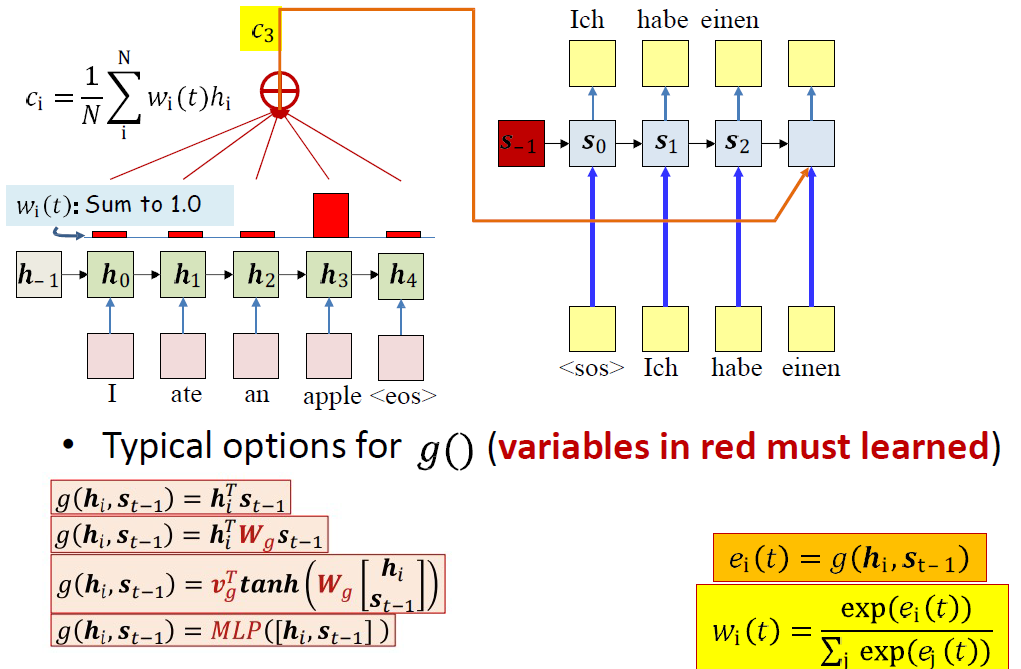
\includegraphics[width=\linewidth, height=0.9\textheight,keepaspectratio]{images/nlp/attention-weights-2.png}
    \end{figure}
    \framebreak
    \begin{figure}
        \centering
        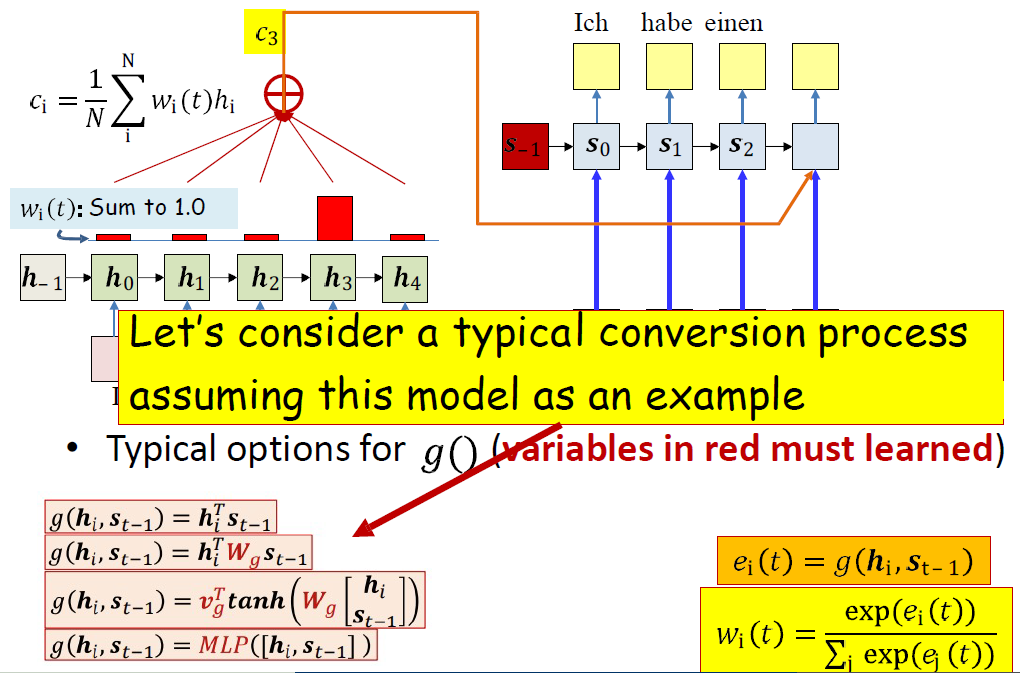
\includegraphics[width=\linewidth, height=0.9\textheight,keepaspectratio]{images/nlp/attention-weights-3.png}
    \end{figure}
\end{frame}

\begin{frame}{Summary: Attention Models}
    \begin{figure}
        \centering
        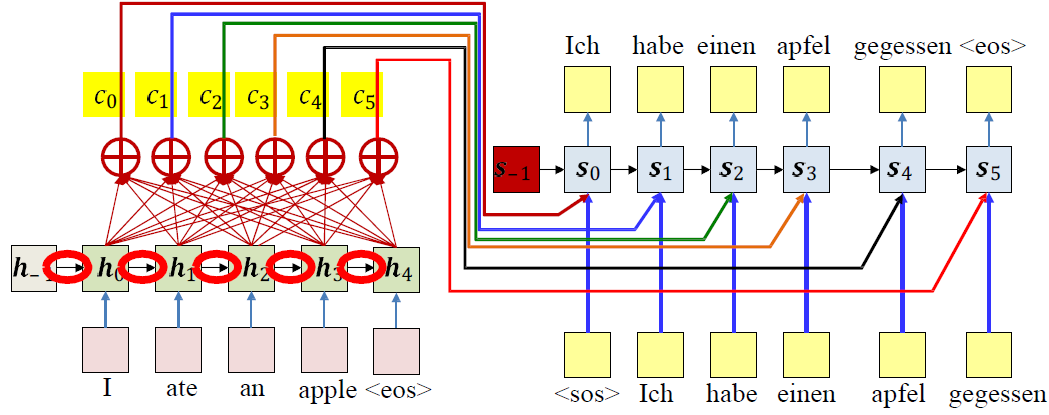
\includegraphics[width=\linewidth, height=0.6\textheight,keepaspectratio]{images/nlp/attention-models-2.png}
    \end{figure}
    \begin{itemize}
        \setlength{\itemsep}{-0.25em}
        \item \textbf{Problem}: The decoder's hidden representation for each output word is influenced by \textit{all} preceding words due to recurrence.
        \item The decoder effectively pays attention to the entire input sequence, not just a single word.
        \item If the decoder can automatically determine which input words to focus on at each step, recurrence in the input may not be strictly necessary.
    \end{itemize}
\end{frame}